\documentclass[11pt]{article}
\usepackage{graphicx}
\newcommand{\numpy}{{\tt numpy}}    % tt font for numpy

\topmargin -.5in
\textheight 9in
\oddsidemargin -.25in
\evensidemargin -.25in
\textwidth 7in

\begin{document}

% ========== Edit your name here
\author{Shi Zuo}
\title{Econ 634 Problem Set 1: Tables and Graphs}
\maketitle

\medskip

% ========== Begin answering questions here
\begin{enumerate}
\section{Answer to Problem 3}
\subsection{Replication result of Table 1 in DGR 2007} 

\begin{figure}[h]
\centering
    \textbf{Quantiles of the 2007 Earnings, Income, and Wealth Distributions ($\times 10^3$ 2007 USD)}\par\medskip
	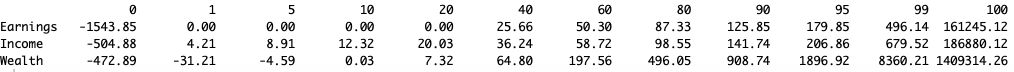
\includegraphics[width=\textwidth]{Table1.png}
\caption{Table 1}
	\label{fig:figure1}
	\end{figure}
	
	
\subsection{Replication result of Table 2 in DGR 2007} 

\begin{figure}[h]
\centering
    \textbf{Concentration and Skewness of the Distributions}\par\medskip
	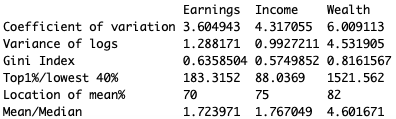
\includegraphics[width=0.5\textwidth]{Table2.png}
\caption{Table 2}
	\label{fig:figure1}
	\end{figure}
\subsection{Lorenz Curve of 2007 Earnings, Income and Wealth}
See next page

\begin{figure}[t]
\centering
   
	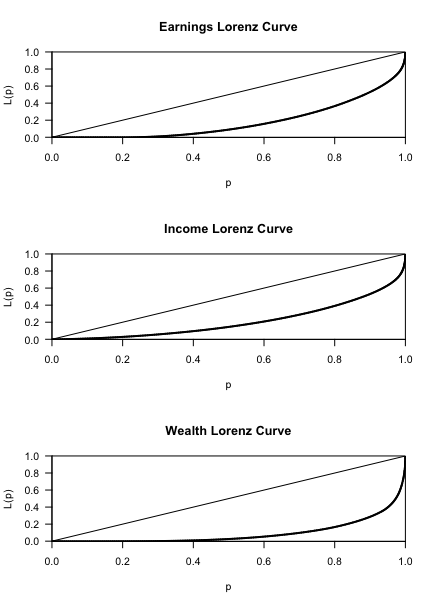
\includegraphics[width=1\textwidth]{LC.png}
\caption{Figure 1}
	\label{fig:figure1}
\end{figure}

% ========== Just examples, please delete before submitting


% ========== Continue adding items as needed


\end{enumerate}
\end{document}
\grid
\grid